\documentclass{beamer}
\usefonttheme[onlymath]{serif}
\usepackage[italian]{babel}
\usepackage{array}
\usepackage{makecell}
\newcolumntype{M}[1]{>{\centering\arraybackslash}m{#1}}
\usepackage{csquotes}
\usepackage{bold-extra}


\begin{document}


\title{Wave Map}
\author{Tian Cheng Xia\\{\footnotesize Matricola: \texttt{975129}}}
\institute{Corso di Laboratorio di applicazioni mobili\\Alma Mater Studiorum -- Università di Bologna}
\date{A.A. 2022 -- 2023}


\begin{frame}
    \titlepage
\end{frame}


\begin{frame}
    \frametitle{Informazioni generali}

    \begin{itemize}
        \item Kotlin
        \item \texttt{Room} per interfacciarsi con il database locale
        \item \texttt{Coroutine} per le operazioni asincrone
        \item Linearizzazione delle funzioni con callback attraverso \texttt{suspendCoroutine}
    \end{itemize}
\end{frame}


\begin{frame}
    \frametitle{Raccolta dati}

    La classe astratta \texttt{WaveSampler} rappresenta un misuratore e richiede l'implementazione dei metodi:
    \begin{itemize}
        \item \texttt{sample}: prende una nuova misurazione
        \item \texttt{store}: salva una misurazione
        \item \texttt{retrieve}: ricerca misurazioni
    \end{itemize}

    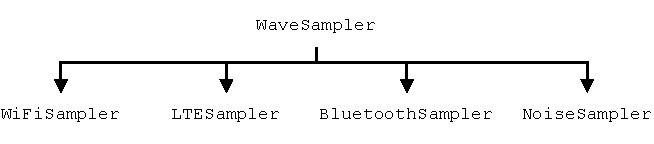
\includegraphics[width=\linewidth]{./img/sampler.pdf}
\end{frame}


\begin{frame}
    \frametitle{Mappa}

    \begin{columns}
        \column{0.65\linewidth}
        \textbf{Cella} descritta dalle coordinate nord-ovest e dalla dimensione in metri.
        \\~\\
        \textbf{Colore} determinato in formato HSL mappando la misurazione nell'intervallo $[0, 150]$ (hue).
        \\~\\
        \textbf{Griglia} generata rispetto ad una celle di riferimento eletta in fase di avvio.

        \column{0.35\linewidth}
        \centering
        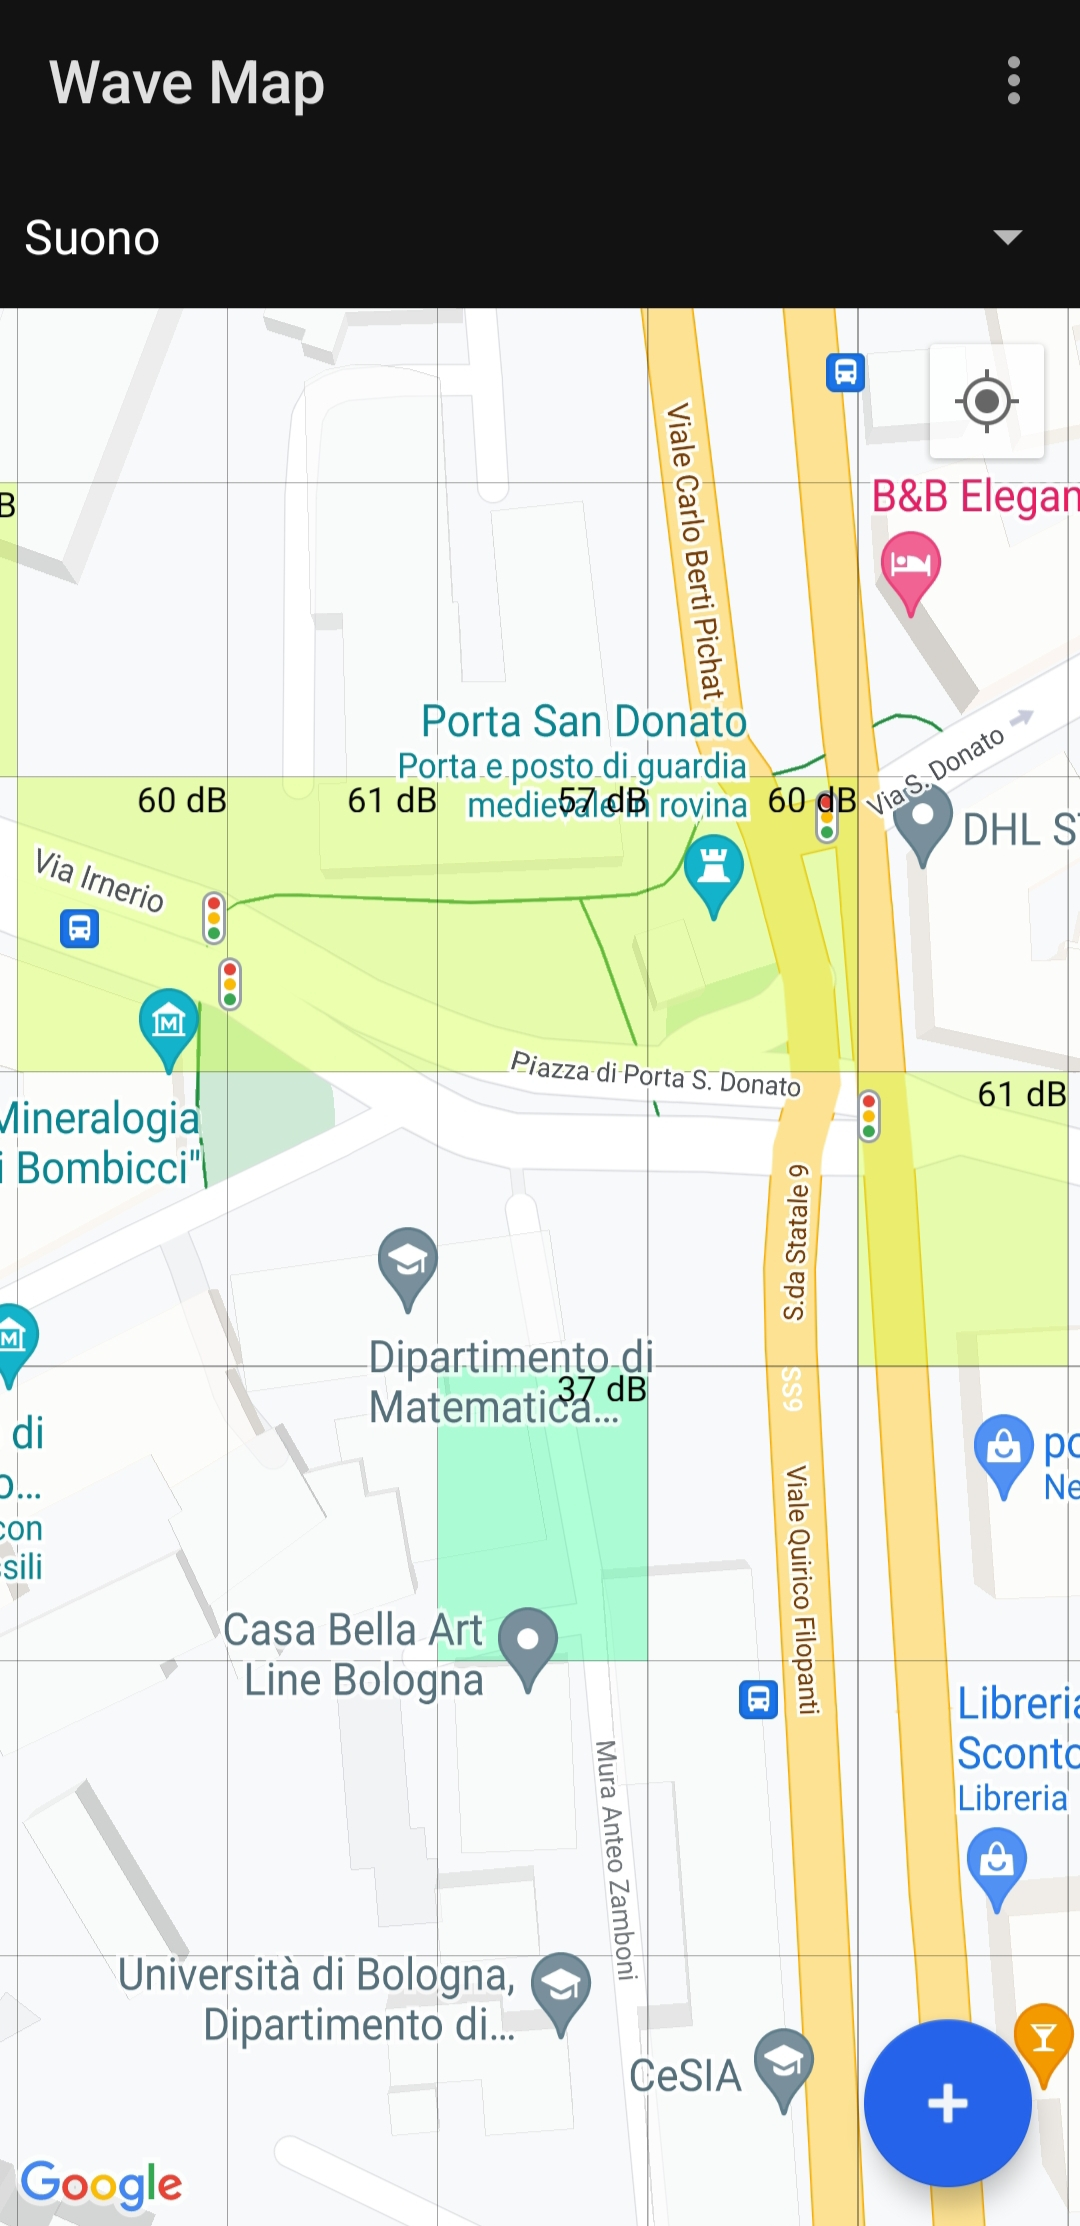
\includegraphics[width=0.90\linewidth]{./img/overview/map_zoom1.jpg}
    \end{columns} 
\end{frame}


\begin{frame}
    \frametitle{App principale}
    \framesubtitle{Overview}

    \centering
    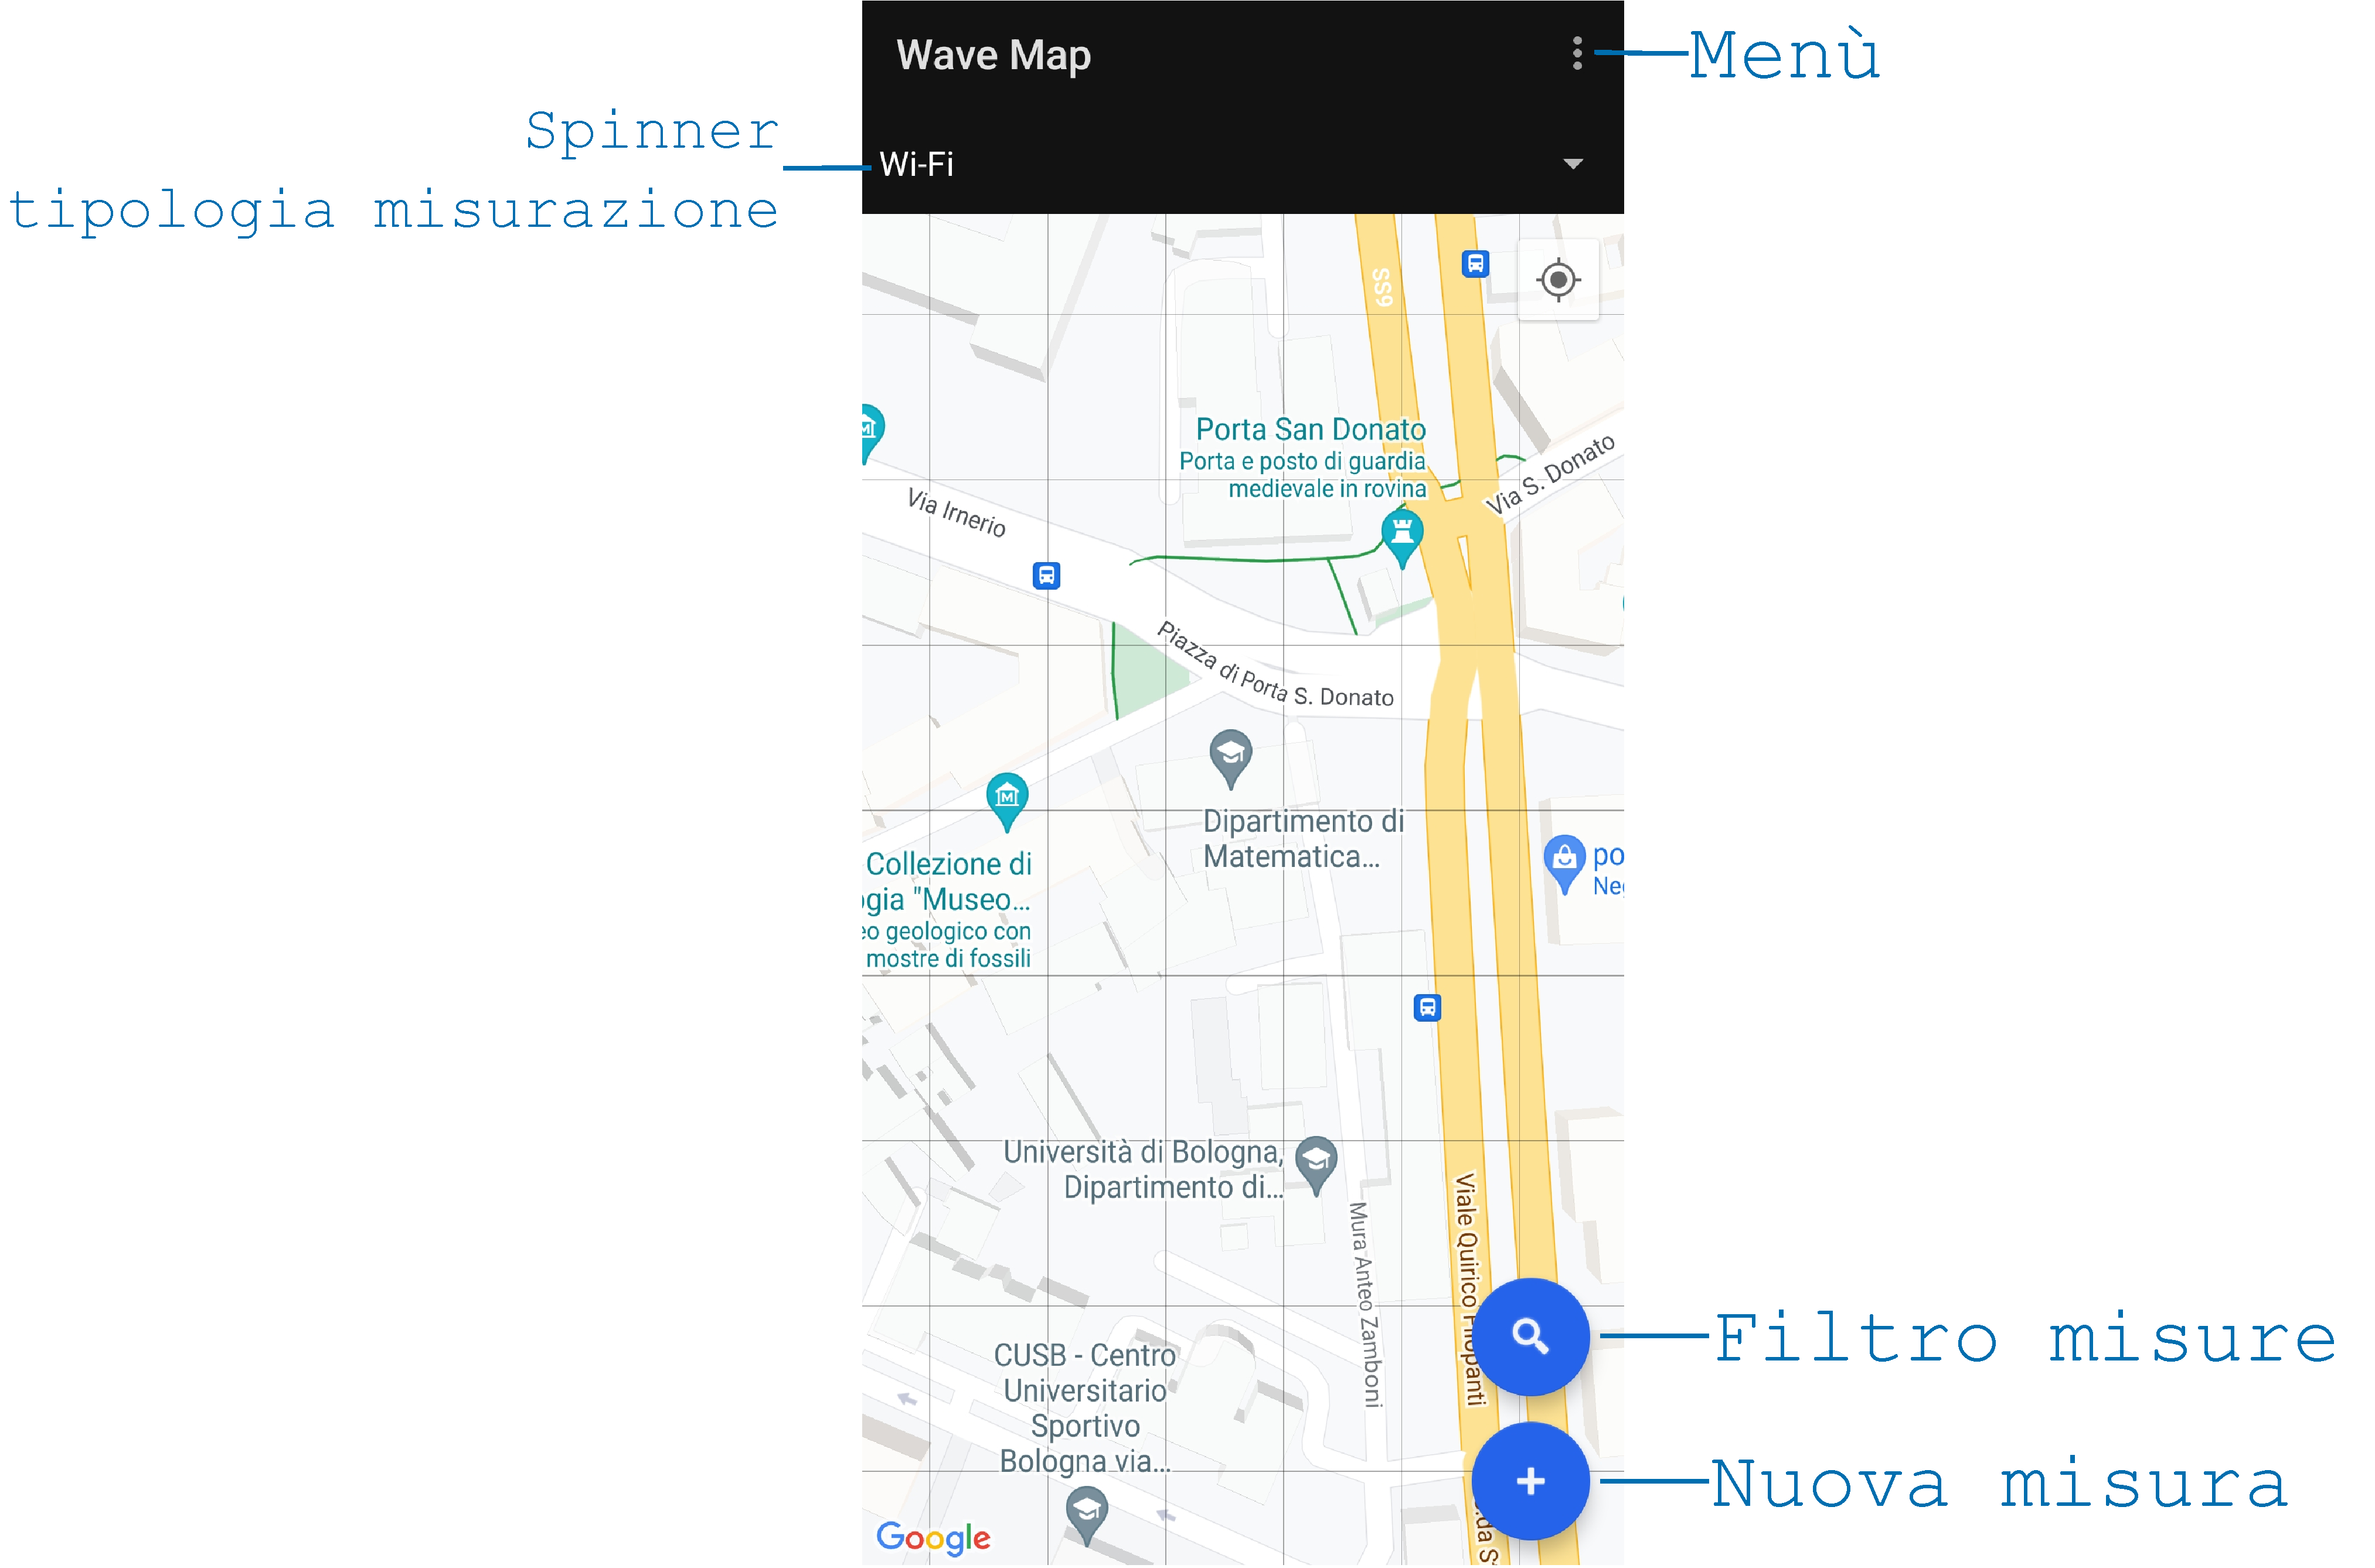
\includegraphics[width=\linewidth]{./img/overview/main.pdf}
\end{frame}


\begin{frame}
    \frametitle{App principale}
    \framesubtitle{ViewModel}

    Ciascun misuratore ha un proprio ViewModel dedicato.
    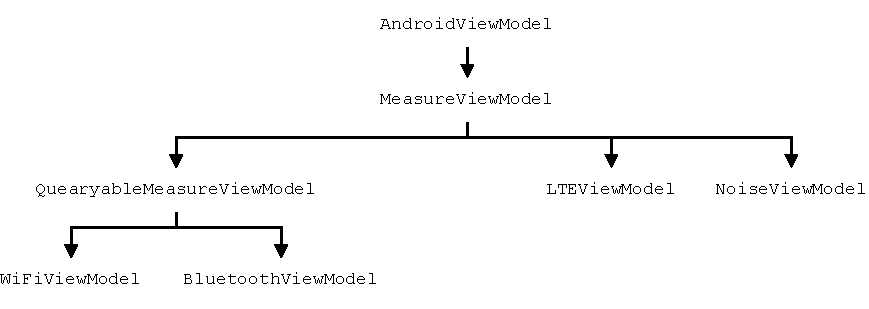
\includegraphics[width=\linewidth]{./img/viewmodel.pdf}

    \textbf{\texttt{MeasureViewModel}} descrive le proprietà base di un misuratore.

    \textbf{\texttt{QueryableMeasureViewModel}} rappresenta un misuratore a cui è applicabile un filtro.
\end{frame}


\begin{frame}
    \frametitle{App principale}
    \framesubtitle{ViewModel}

    Il ViewModel principale è \texttt{MainViewModel}.
    \begin{itemize}
        \item Contiene un'istanza di ciascun ViewModel dei misuratori
        \item Gestisce il misuratore attualmente attivo
        \item Garantisce mutua esclusione per ciascun misuratore
        \item \texttt{LiveData} per notificare la view dei cambiamenti
    \end{itemize}
    

\end{frame}


\begin{frame}
    \frametitle{Impostazioni}

    \begin{columns}
        \column{0.65\linewidth}
        Creata utilizzando la libreria \texttt{Preference}.
        \\~\\
        Ciascun misuratore ha una pagina dedicata generata dinamicamente.

        \column{0.35\linewidth}
        \centering
        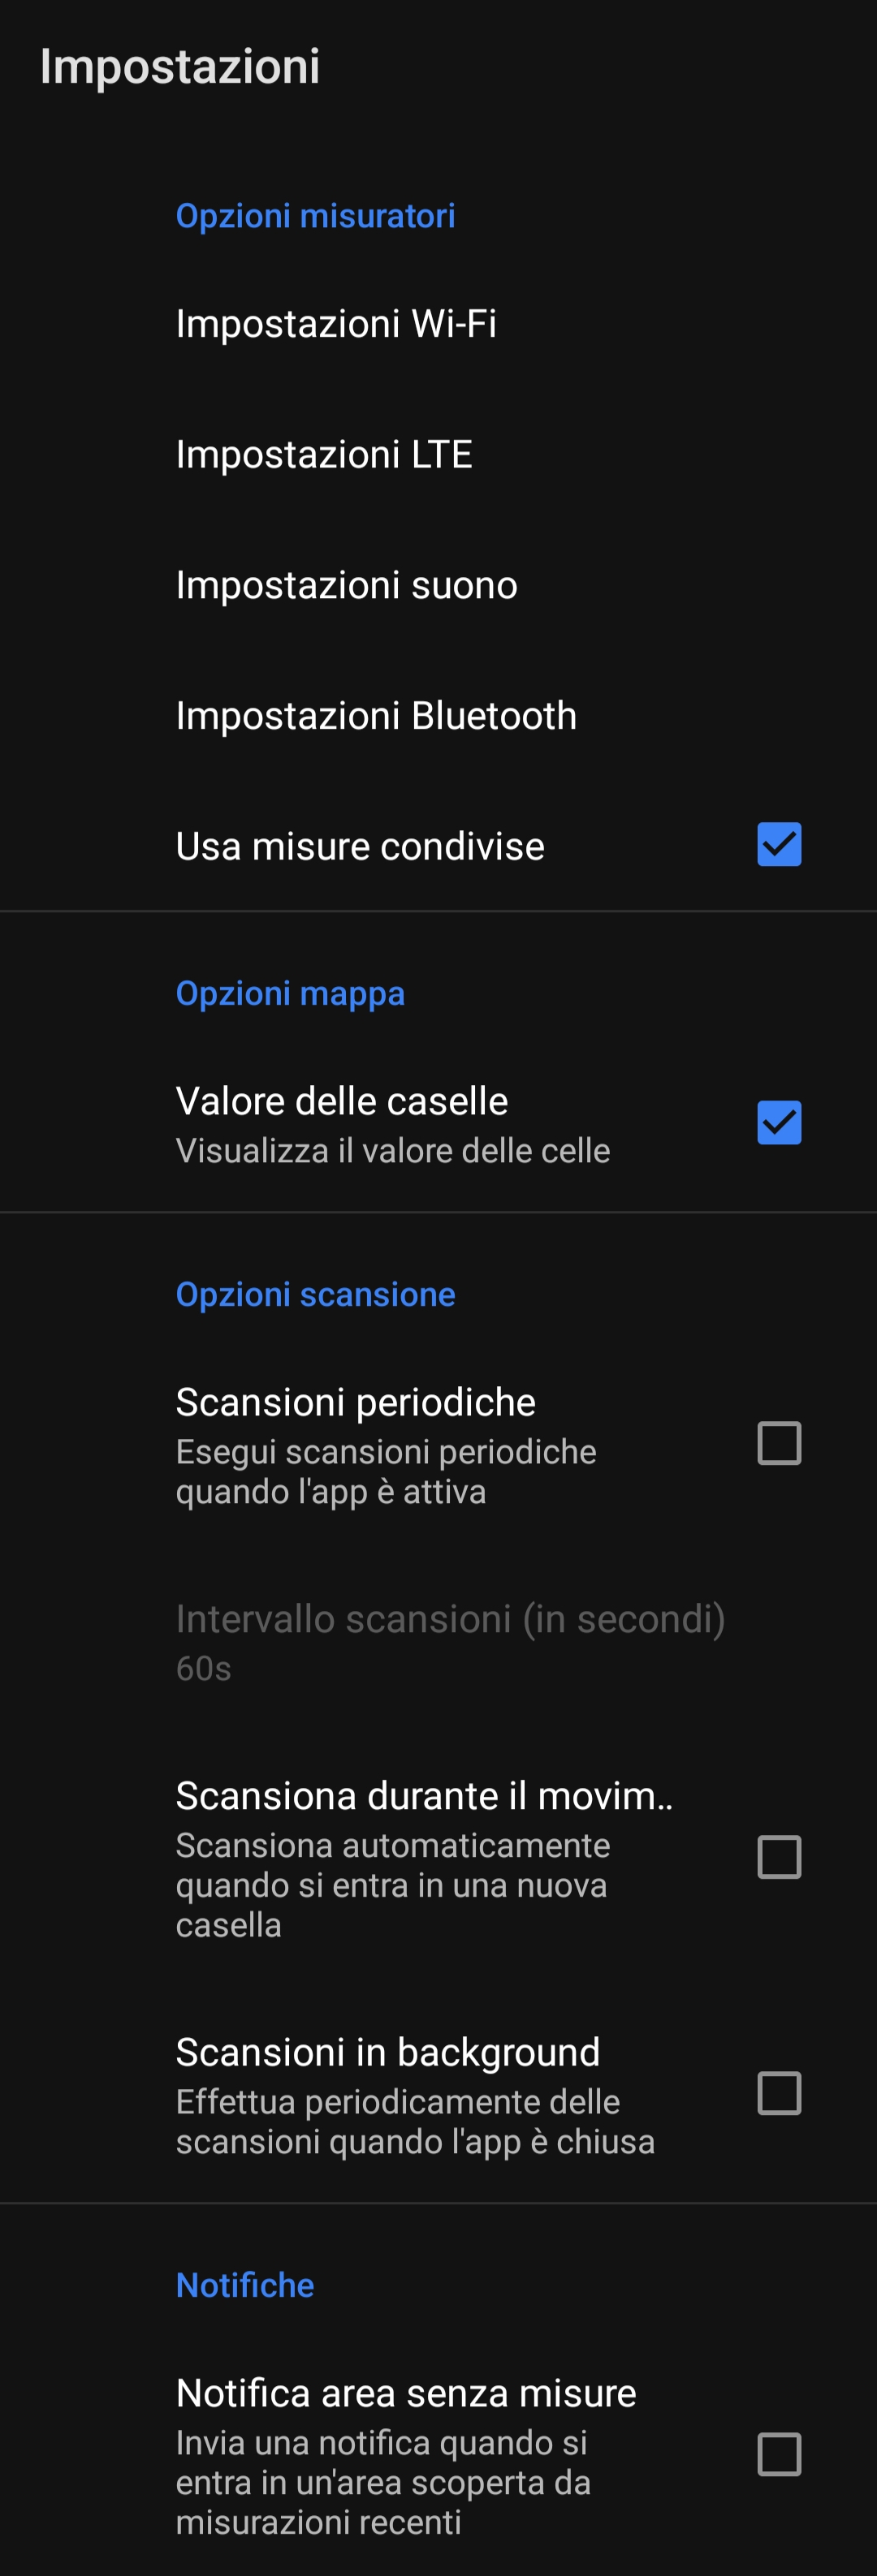
\includegraphics[width=0.70\linewidth]{./img/overview/settings1.jpg}
    \end{columns} 
\end{frame}


\begin{frame}
    \frametitle{Servizio in background}

    \begin{itemize}
        \item Scansioni durante il movimento
        \item Notifica di aree prive di misurazioni recenti
    \end{itemize}

    Il servizio viene avviato come \textit{Foreground Service} se è necessario effettuare scansioni.

    \begin{figure}[H]
        \raisebox{-0.5\height}{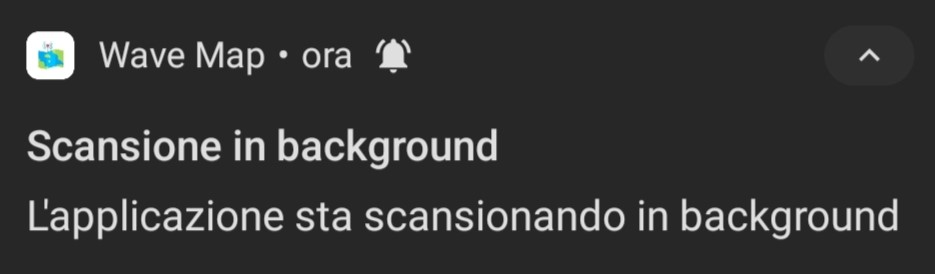
\includegraphics[width=0.40\textwidth]{./img/overview/notification_scan.jpg}}
        \hspace*{1cm}
        \raisebox{-0.5\height}{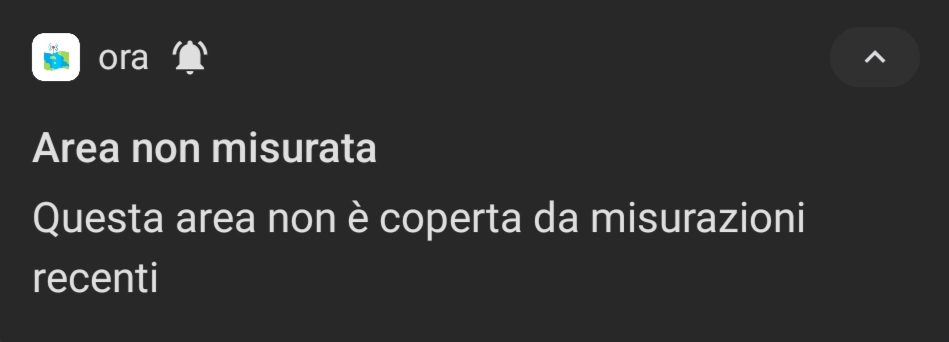
\includegraphics[width=0.40\textwidth]{./img/overview/notification_uncovered.jpg}}
    \end{figure}
\end{frame}


\begin{frame}
    \frametitle{Condivisione dati}

    Esportazione su file in formato JSON.

    Importazione attraverso \texttt{intent-filter}.

    \begin{figure}[H]
        \centering
        \begin{minipage}[b]{0.25\textwidth}
          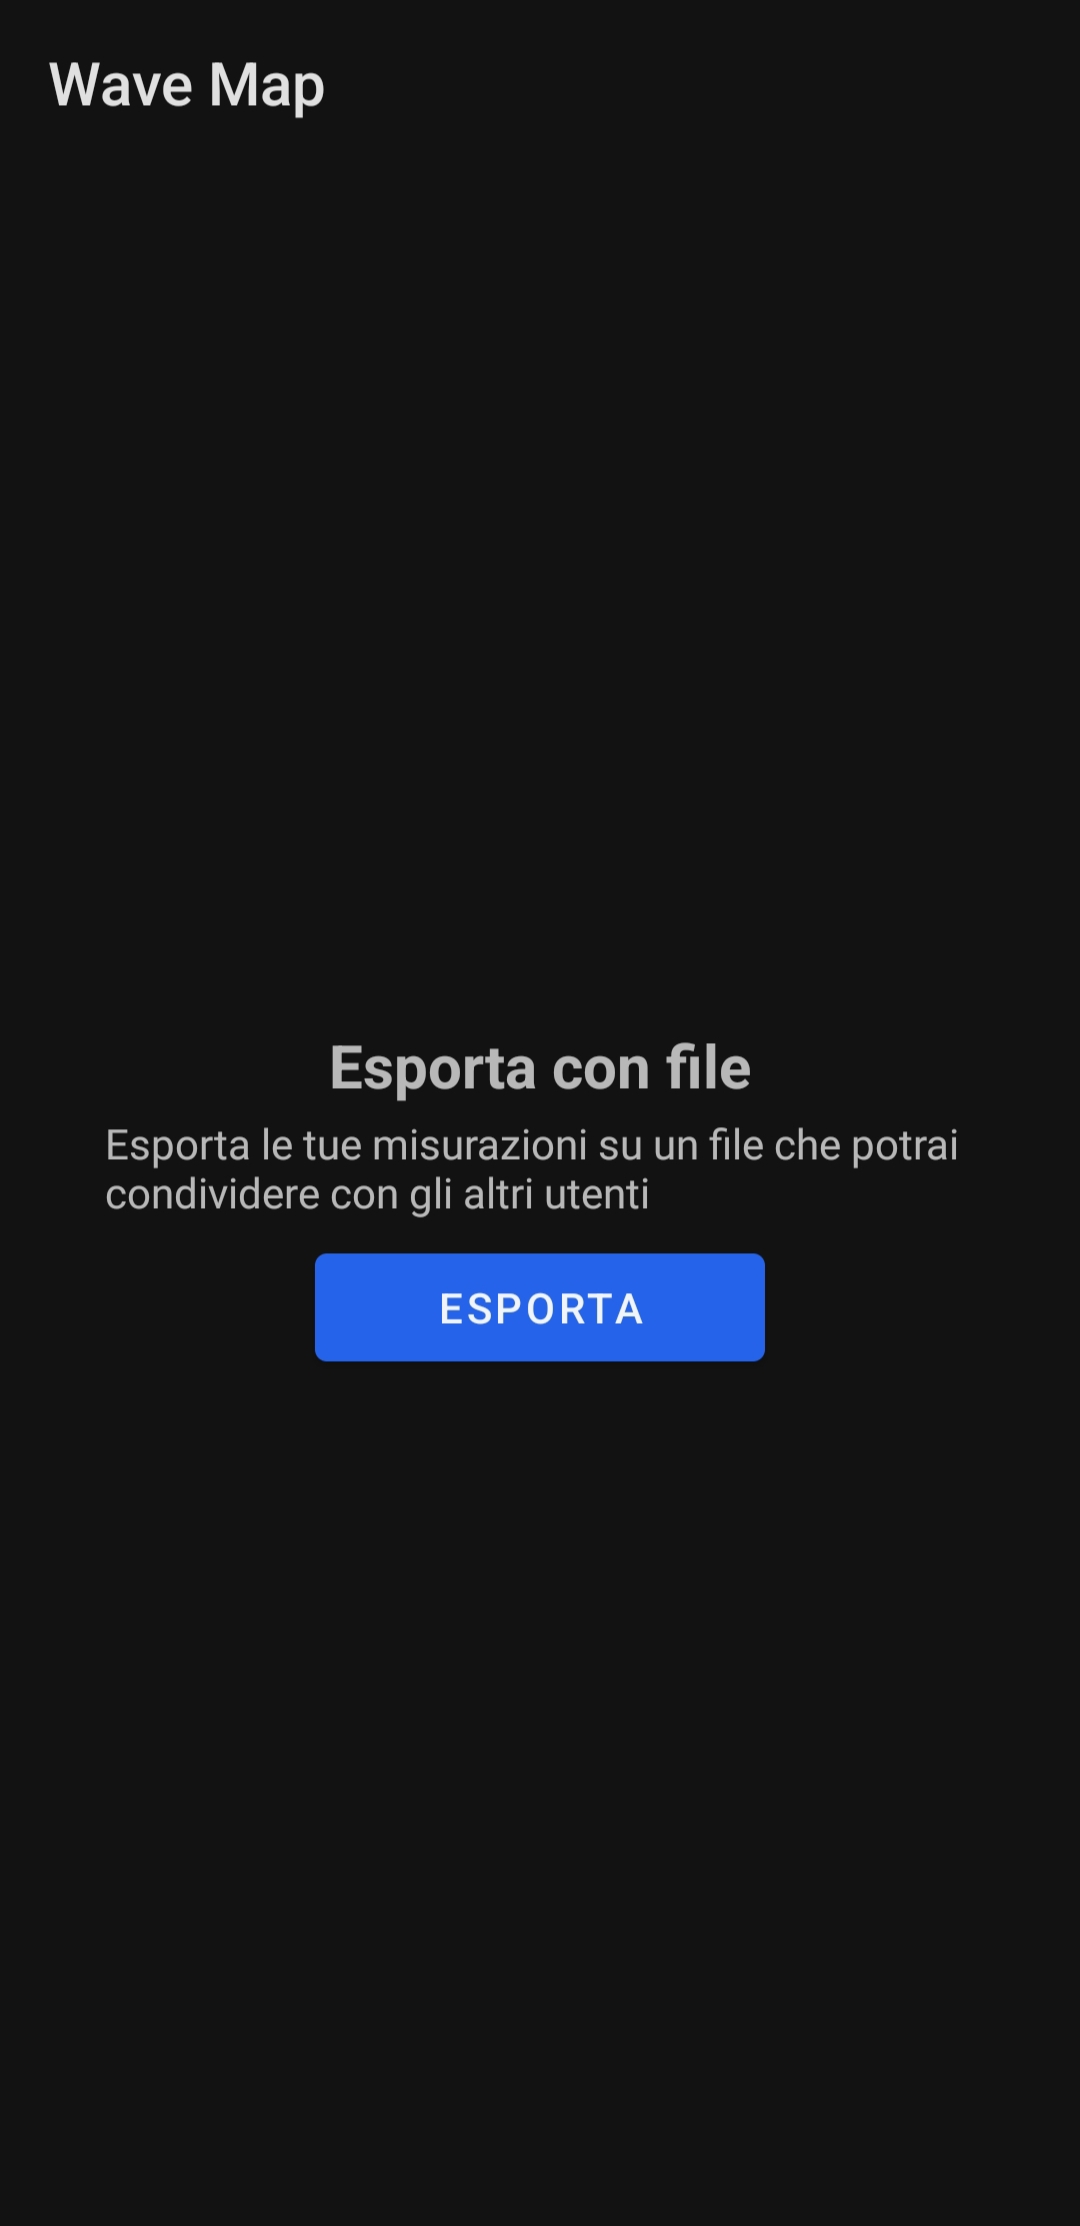
\includegraphics[width=\textwidth]{./img/overview/export1.jpg}
        \end{minipage}
        \begin{minipage}[b]{0.25\textwidth}
          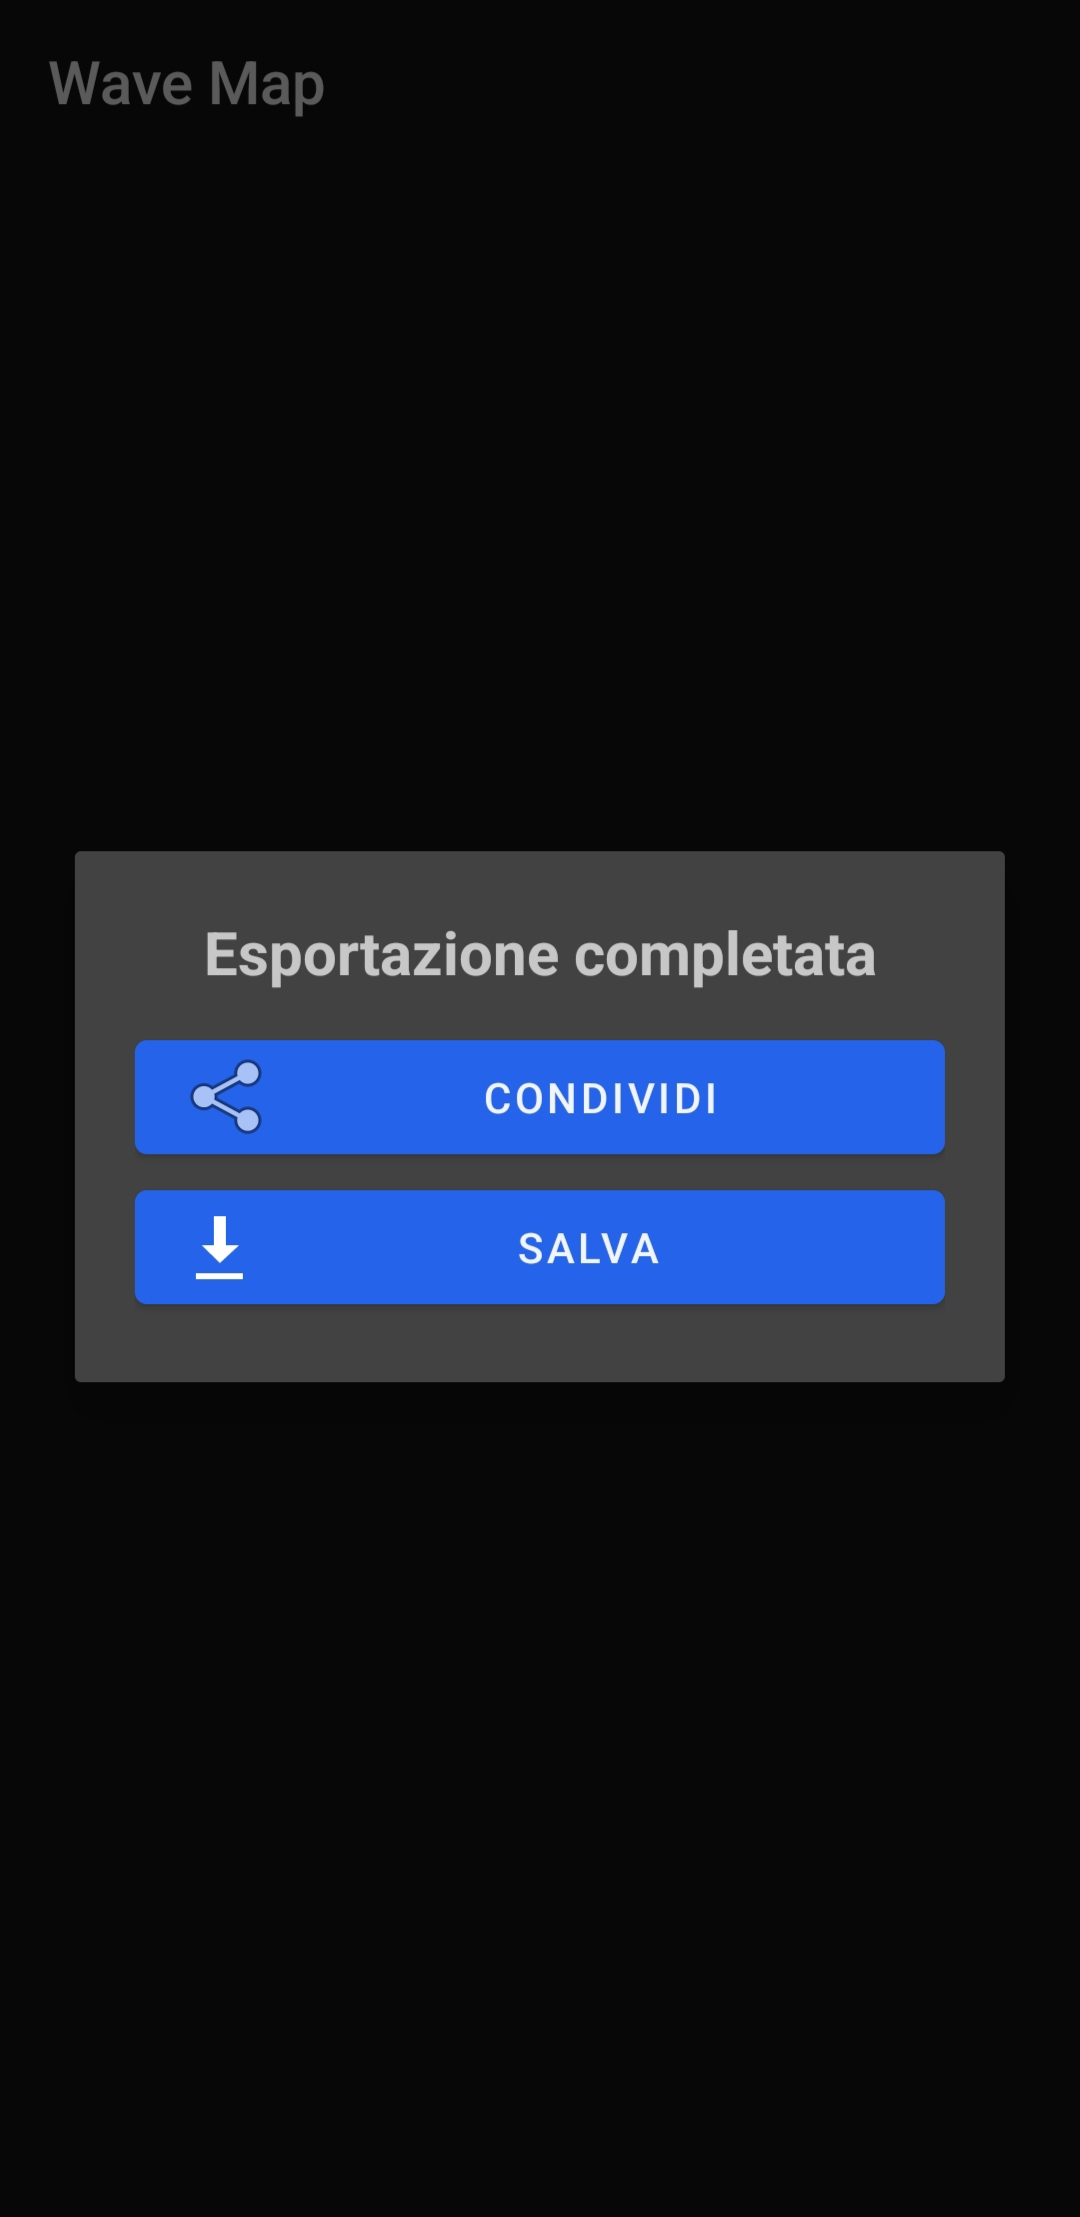
\includegraphics[width=\textwidth]{./img/overview/export2.jpg}
        \end{minipage}
        \hspace*{1cm}
        \begin{minipage}[b]{0.25\textwidth}
          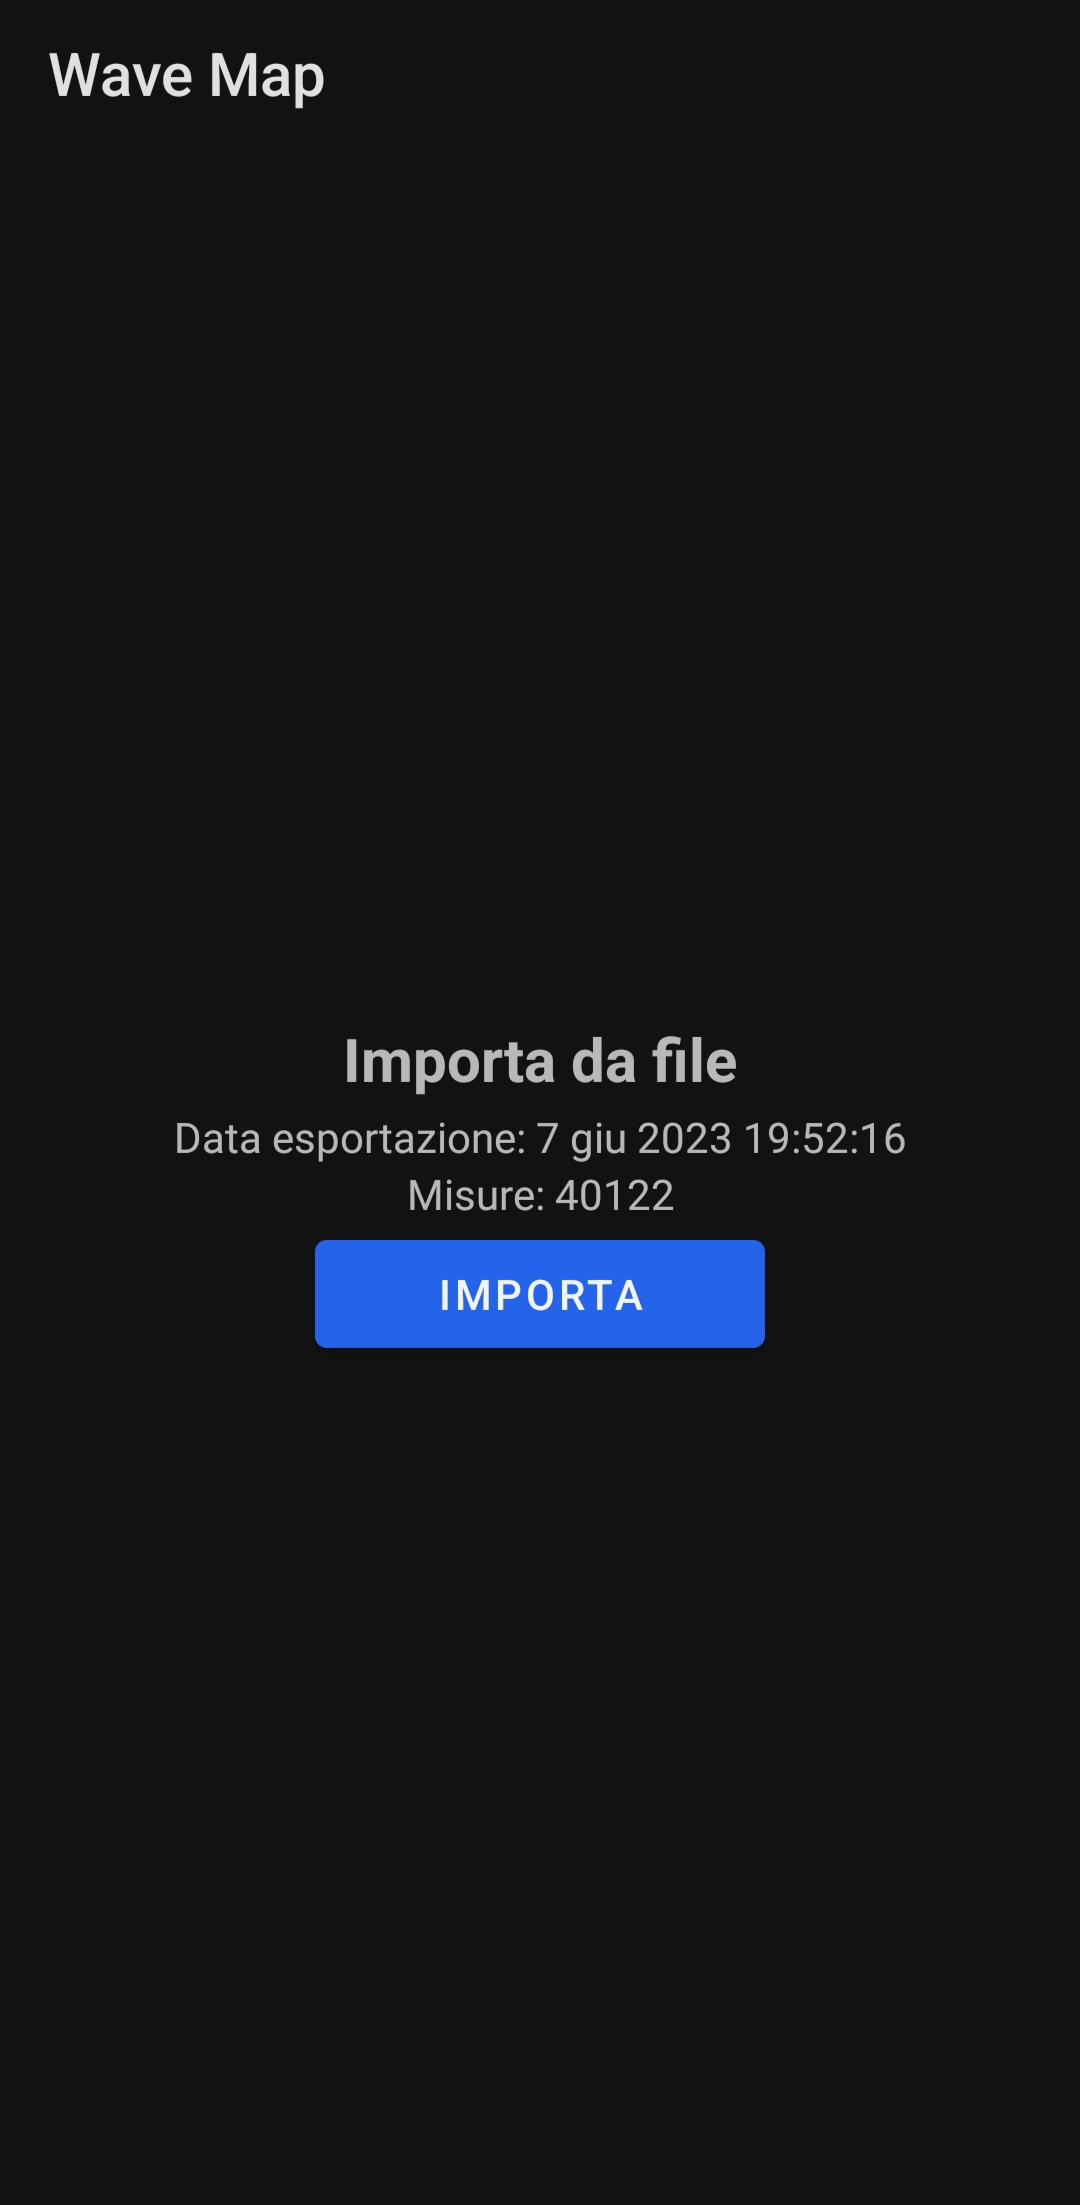
\includegraphics[width=\textwidth]{./img/overview/import.jpg}
        \end{minipage}
    \end{figure}
\end{frame}



\begin{frame}
    \frametitle{Problemi noti}

    \begin{itemize}
        \item Dall'API 26 sono state introdotte restrizioni al numero di scansioni Wi-Fi che un'applicazione può fare
        \item Alcuni produttori hanno politiche di ottimizzazione della batteria che tendono a limitare i servizi in background
        \item L'\texttt{intent-filter} per l'importazione ammette input che non necessariamente riguardano l'app
    \end{itemize}
\end{frame}

\end{document}